\chapter{An automated, objective and open source tool for stream threshold selection and upstream riparian corridor delineation}
\label{chapter2}

Avit Kumar Bhowmik\textsuperscript{a}, Markus Metz\textsuperscript{b} and Ralf B. Schäfer\textsuperscript{a}\\[.5cm]
\small
\textsuperscript{a}Quantitative Landscape Ecology, Institute for Environmental Sciences, University of Koblenz-Landau, Fortstraße 7, 76829 Landau in der Pfalz, Germany\\
\textsuperscript{b}GIS and Remote Sensing Platform, Biodiversity and Molecular Ecology Department, Research and Innovation Centre - Fondazione Edmund Mach, Via E. Mach 1, 38010 - S. Michele all’Adige (TN), Italy\\[1cm]
\medskip
\normalsize
Adapted from the article published in 2015 in Environmental Modelling \& Software\footnote{Environmental Modelling \& Software is one of the most important scientific journals in the field of environmental models, software, tools and methods development. The current impact factor of the journal is 4.420 according to the Journal Citation Reports, 2015 (\href{http://wokinfo.com/products_tools/analytical/jcr/#}{http://wokinfo.com/products\textunderscore tools/analytical/jcr/#})}, vol. 63, pp 240-250.\\[.5cm]

\renewcommand{\abstractname}{Abstract}
\begin{abstract}
The extraction of stream networks from digital elevation models (DEM) and delineation of upstream riparian corridors (URC) for stream sampling points (SSP) are frequently used techniques in freshwater and environmental research. Selection of an accumulation threshold (AT) for stream extraction and delineation of URCs are often done manually. Two algorithms are introduced in this paper that allow for automated AT selection and URC delineation. ATs are selected to yield the highest overlap of DEM-derived and traditionally mapped streams as well as to assure extraction of all mapped streams from DEMs. URCs are delineated after snapping SSPs to DEM-derived streams. The new tool showed similar or better performance than comparable algorithms and is freely available, interfacing the open source software packages R and GRASS GIS. It will improve the extraction of stream networks and the assessment of magnitude and scale of effects from riparian stressors (e.g. land use) on freshwater ecosystems. 
\end{abstract}

\newpage
\thispagestyle{empty}

\vspace*{\fill}
\begin{quotation}
\centering
  \large\textit{``You never change things by fighting the existing reality. To change something, build a new model that makes the existing model obsolete''}.
   ---Buckminster Fuller
\end{quotation}
\vspace*{\fill} 

\newpage

\section{Introduction}
\label{introduction}

The increasing availability of high quality digital elevation models (DEM) has advanced the automatic extraction of stream networks (DeVantier and Feldman, 1993). Extraction of streams from DEMs often achieves higher accuracy, precision and efficiency than mapping by traditional field survey and historical map digitization (Moore et al., 1991; Olivera, 2001). Moreover, DEM-derived stream networks (DSN) are topologically clean and homogenous. Therefore, they have largely been applied in modeling abundance and distribution of aquatic communities (Moore et al., 2000; Narumalani et al., 1997) and geo-computation on physiochemical processes, i.e. carbon flux and greenhouse gas emission in streams (Teodoru et al., 2009). DSNs are also more suitable for the calculation of hillslope travel distances (Ogden et al., 2001) and for the measurement of hydrological proximities (Tesfa et al., 2011) than traditionally mapped stream networks (MSN).

Extracted DSNs also allow for simple determination of different hydrological features from corresponding DEMs such as flow direction, catchment size, stream density, stream order and stream flow periodicity (Gichamo et al., 2012; Hughes et al., 2011). These features are useful tools in many fields of freshwater research, e.g. cartography, geomorphology, ecology and water resources management. For example, catchment size, drainage density and stream orders provide important information for fluvial geomorphological studies and thus help in deriving hydrograph and sediment production that depict suitability of a region for agriculture and urbanization (Berhane and Walraevens, 2013; Maidment et al., 1996). Water resources management practices can benefit from accurate and homogenous mapping of temporary streams and can eventually contribute to restoring habitats of aquatic communities (Wang et al., 2002). Moreover, stream orders and catchments are useful for flood and non-point source pollution modeling (Di Luzio et al., 2004), assessing economic values of riverine land parcels (Bastian et al., 2002) and planning for construction works (Forman, 2003).

Numerous geographic information system (GIS) tools enable DSN extraction, among them “r.watershed” (Metz et al., 2011) and “r.stream” (Jasiewicz and Metz, 2011) in GRASS GIS (GRASS Development Team, 2014), and “ArcHydro” (Maidment, 2002) and “TauDEM” (Tarboton, 2005) in ArcGIS (ESRI, Redlands, 2001) and QGIS (QGIS Development Team, 2014) are widely applied. These tools extract DSNs by four consecutive steps: i) pit removal, ii) flow direction raster computation, iii) flow accumulation raster computation and iv) extracting streams as cells exceeding an accumulation threshold (AT) (see Tarboton et al. (1991) for terminologies). The first three steps are largely automated  (Arge et al., 2003; Danner et al., 2007; Garbrecht and Martz, 1997; Tarboton, 2005), whereas the AT for distinguishing between stream and non-stream cells is often set arbitrarily and then DSNs are manually (visually) compared to MSNs (Tarboton et al., 1991). This manual procedure via trial and error may either result in too many (non-existing) streams (lower AT than optimal) or miss streams or stream stretches (higher AT than optimal) (Montgomery and Foufoula-Georgiou, 1993). In addition, this procedure is laborious. 

Values of AT vary according to the scale of studies, i.e. larger scale studies require higher order streams and thus higher AT values and vice versa (Tarboton, 2005). However, the AT selected for a large scale study using a low resolution DEM might also be suitable for a small scale study using a high resolution DEM. A few stream network extraction algorithms using automated AT consider the scale of studies (resolution of DEMs) but do not compare DSNs with MSNs. These algorithms compute ATs by (1) slope-area power links (Montgomery and Foufoula-Georgiou, 1993) and (2) stream drop analysis, i.e. statistical significance of the difference between extracted first and higher order streams (Tarboton, 2005). However, ATs computed by these algorithms require further validation with respect to geomorphology, soil and climate of the study area as they strongly affect actual stream initiation, as well as by available MSNs (Lin et al., 2006).

Many studies require extraction of DSNs that approximate given MSNs, e.g. fitting statistical and geo-statistical models to the observations on MSNs that require hydrological parameters from DEMs (as done by “STARS” (Peterson and Ver Hoef, 2014), “SSN” (Ver Hoef et al., 2012) and “rtop” (Skøien et al., 2014)), catchment extraction from DEMs for outlets defined on MSNs (Hofierka et al., 2009; Tarboton, 2005) and DEM-based geo-computation on the processes that are observed in MSNs (Lagacherie et al., 2010). Hence, a few studies automated the AT selection process through comparison with MSNs, also considering the scale of MSNs. These automation are based on (1) statistical relations with landscape parameters at stream sources of MSNs (Heine et al., 2004) and (2) minimizing lateral displacements ($d$) between stream sources of MSNs and DSNs (Lin et al., 2006). However, algorithms relying on landscape parameters are highly demanding in terms of input data and computation. The minimized lateral displacement between mapped and DEM stream sources may result from non-existing streams related to a low AT. Consequently, the number of DEM-derived streams should be considered during optimization. Furthermore, lateral displacements are often observed between MSNs and DSNs due to differences in data sources, equipment and human processing, which leads to imprecision in the selection of mapped stream sources and outlets from DEM (Peterson and Ver Hoef, 2014; Soille et al., 2003). This may consequently hinder the extraction of an approximate DSN. The suggested solution of “burning in’’ MSNs (Maidment et al., 1996; Peterson and Ver Hoef, 2014) alters DEMs and may affect subsequent analyses (Callow et al., 2007).

The advent of high quality DEMs also allows for the delineation of riparian corridors for streams and stream sections of DSNs by geomorphological analyses (Abood et al., 2012; Fernández et al., 2012; Holmes and Goebel, 2011). The land cover in riparian corridors interacts with many processes within streams and has a strong influence on water quality and energy fluxes (Verry et al., 2004). Therefore multiple stressors that act on riparian scales also affect stream communities and processes (Marzin et al., 2013). However, communities and processes in streams are typically monitored at stream sampling points (SSP) in governmental monitoring programs (Biss et al., 2006). The SSPs are ideally representative for the whole stream network and usually physicochemical variables such as pH and temperature as well as biological quality elements such as fish or invertebrates are monitored (Stevens Jr and Olsen, 2004). Hence, SSPs can be used to quantify potential effects from riparian scale stressors on the biological endpoints (e.g. community composition of invertebrates). This in turns requires computation of upstream riparian corridors (URC) of given sizes (length and width), for which these stream sampling points serve as outlets (Dahm et al., 2013; Lorenz and Feld, 2013; Marzin et al., 2013). To our knowledge, no algorithm has been developed for automated delineation of such URCs for given SSPs and sizes. To date such corridors are often “drawn by hands” (Colson et al., 2008).

Moreover, the available algorithms for automated AT selection and riparian corridor delineation for streams and stream sections were mostly developed on proprietary software and hence are not accessible. The development of comparable open source software algorithms has been suggested to improve reproducibility, reliability and communication in geoscientific research (Rocchini and Neteler, 2012; Steiniger and Hay, 2009).

Two novel algorithms are presented in this paper: 1) automated AT selection that objectively approximate DSNs to given MSNs and (2) automated URC delineation for given SSPs and sizes from governmental biomonitoring data.    The combination of the two algorithms is called “automated Accumulation Threshold computation and RIparian Corridor delineation (ATRIC)”. ATRIC has been developed by combining two freely available open source software packages. ATRIC is compared with other available algorithms regarding the goodness of DSNs, and its computational efficiency and potential fields of application are discussed.

\section{Materials and Methods}
\label{materials and methods}

\subsection{Data and software}
\label{data and software}

ATRIC was applied on two spatial scales (extent): i) small watershed scale (northeast of the German state Hessen, area 45 km\textsuperscript{2}) and ii) large scale (the German state Thüringen, area 16,171 km\textsuperscript{2} and 100 watersheds) (Figure 2.1). Both regions are characterized by a complex topography composed of flat, valley and hilly lands (HMUELV, 2013; TMLFUN, 2013). The mapped stream networks (MSN) and stream sampling points (SSP, 4 and 1010, respectively) were obtained from governmental biomonitoring (Biss et al., 2006) in these regions. These data were collected from the departments of environment, geology and agriculture of the state authorities of Hessen (HMUELV, 2013) and Thüringen (TMLFUN, 2013). The stream networks were mapped by physical feature surveys by the state authorities and were validated against digital landscape models, digital orthophotos and official land registers. The digital elevation models (DEM) for both regions were the ASTER GDEM with 25 m resolution (NASA and METI, 2009).

\noindent\begin{figure}[h!]
  \centering
  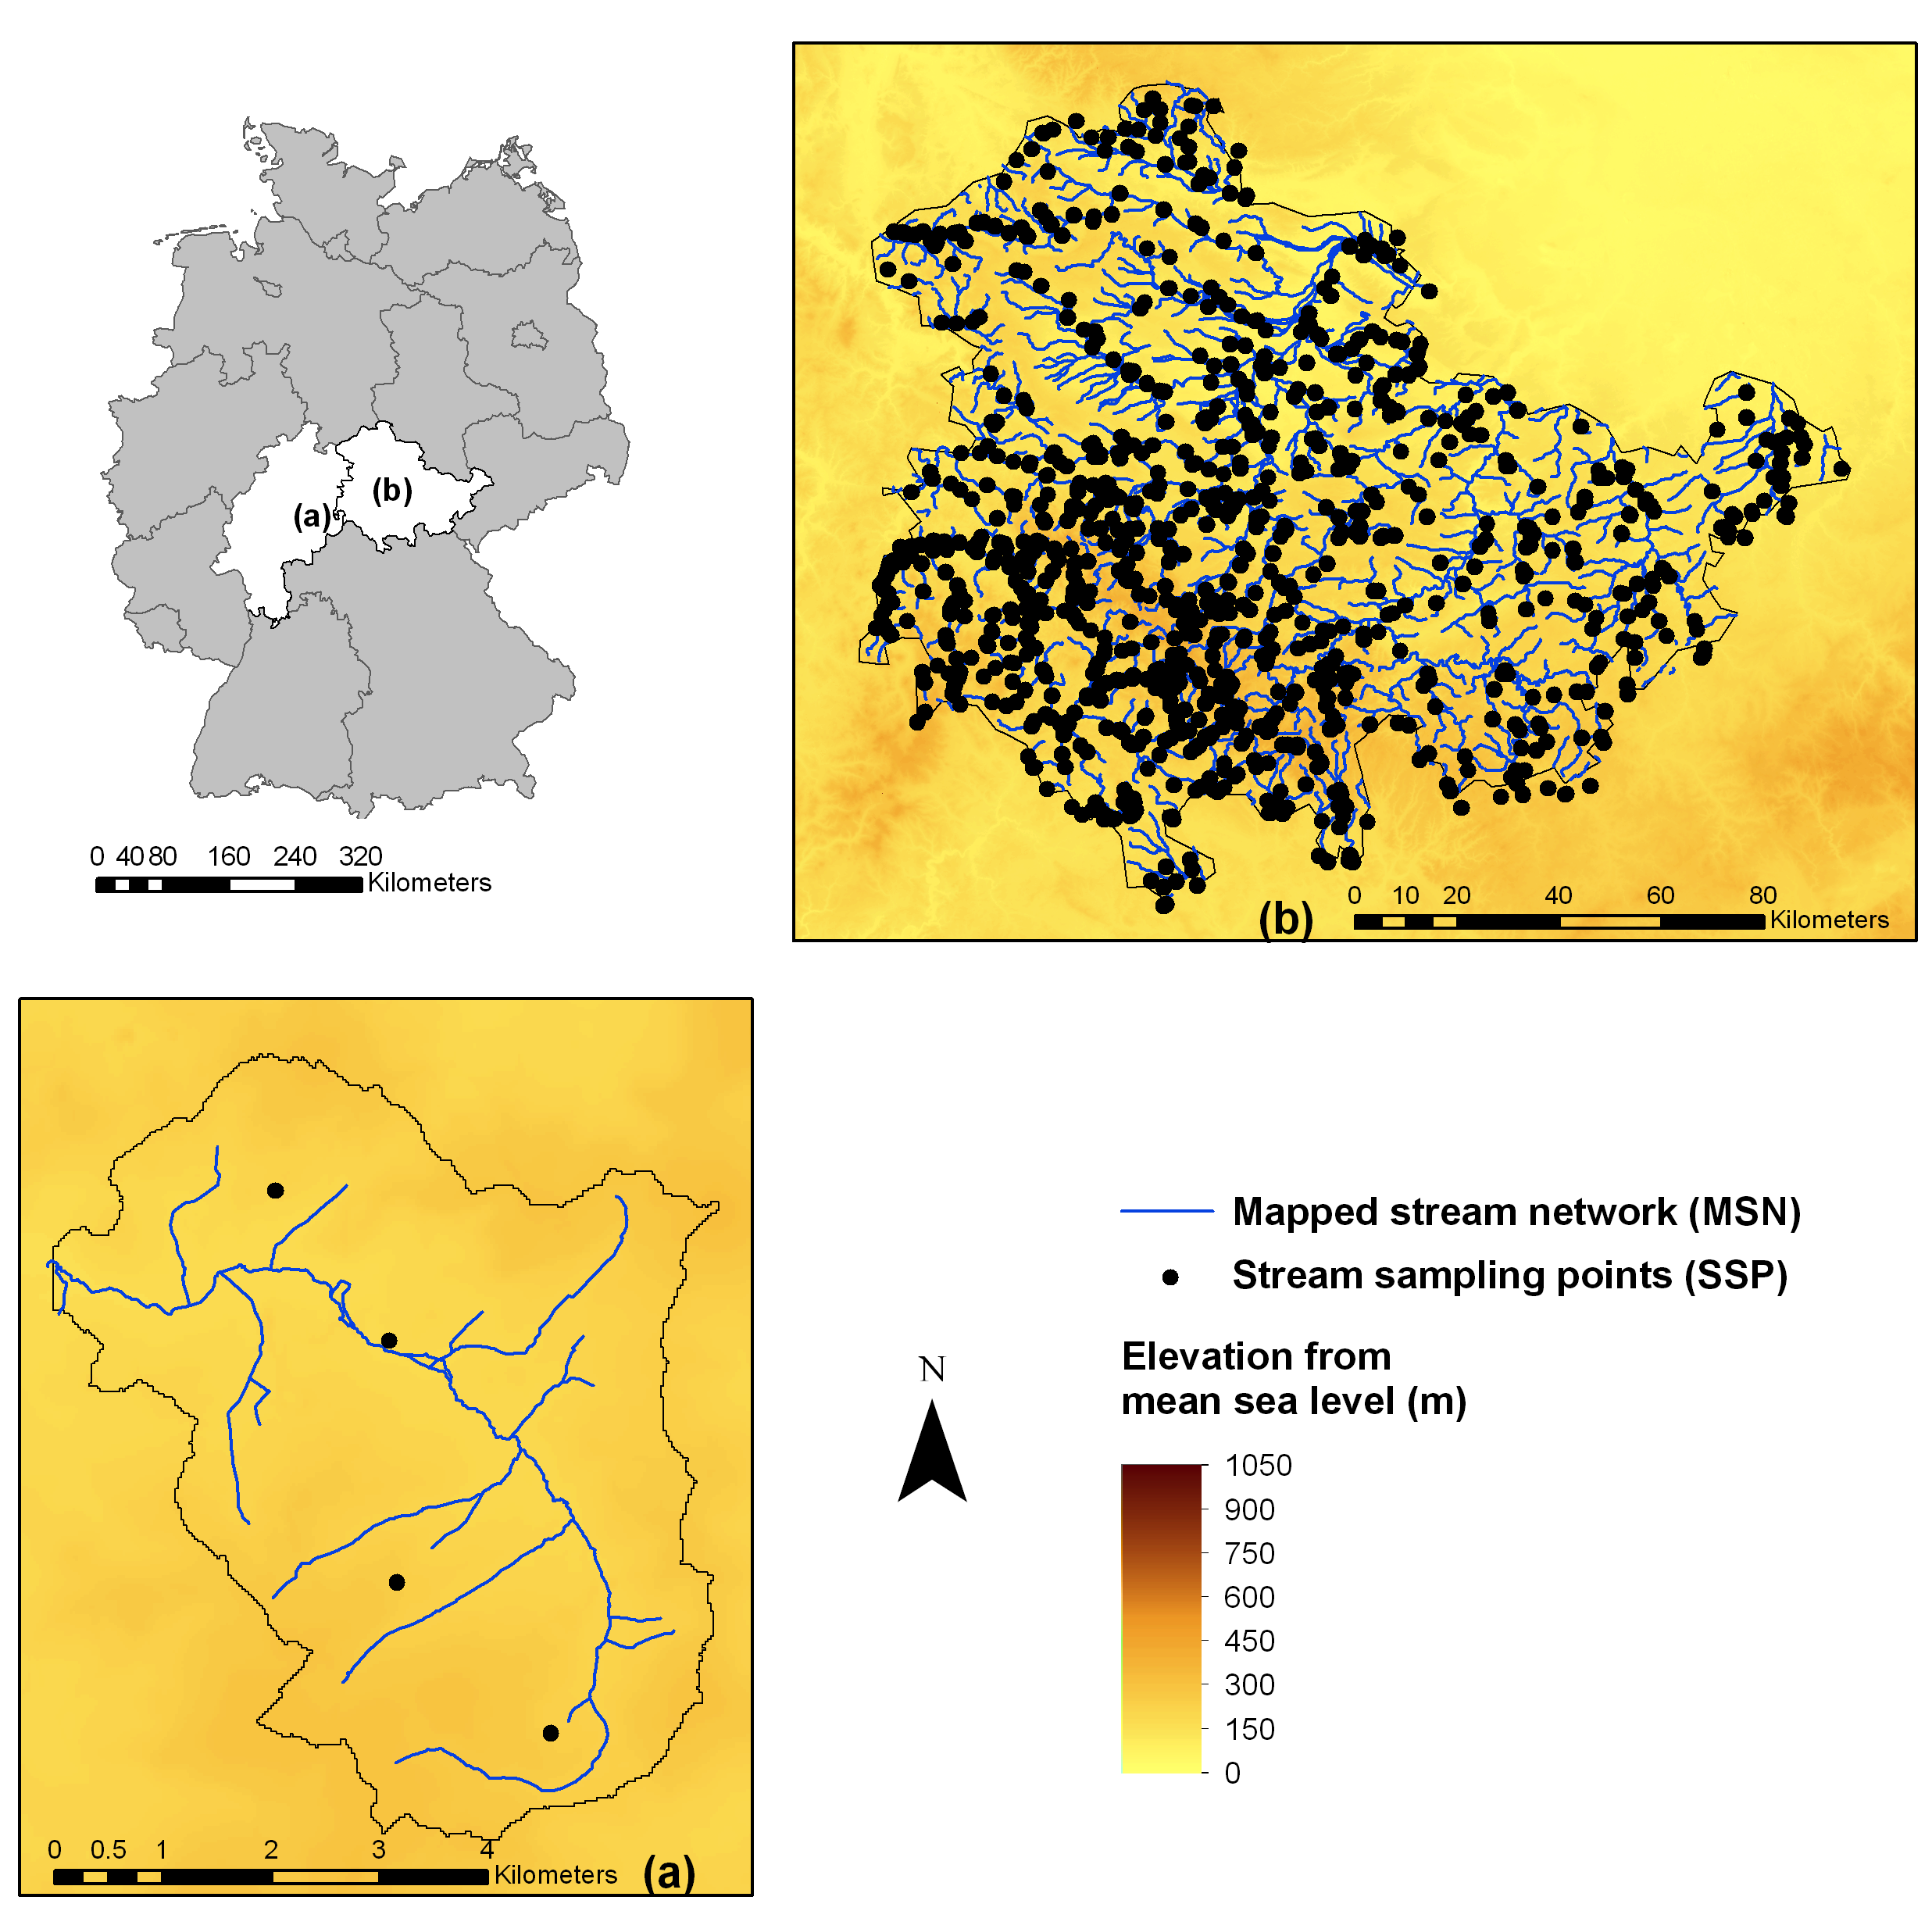
\includegraphics[width=\textwidth]{Figures/Fig_2_1.png}
  \caption{The digital elevation models (DEM) (in the background), mapped stream networks (MSN) and stream sampling points (SSP) in the (a)  watershed at  northeast of German state Hessen and (b) German state Thüringen. The inset represents the included states on a German administrative map. Details of the spatial reference system: coordinate system- Gauss Krüger, projection- Transverse Mercator, datum- Deutsches Hauptdreiecksnetz and units- Meter. Data source: HMUELV (2013), NASA and METI (2009) and TMLFUN (2013).}
  \label{Fig_2_1}
\end{figure}

ATRIC was implemented using R (R Core Team, 2014) with an interface to GRASS GIS (GRASS Development Team, 2014), i.e. the package “spgrass6” that allows for running GRASS GIS modules from the R environment (Bivand, 2007). The other used R packages were- “raster” (Hijmans and Van Etten, 2010), “rgdal” (Keitt et al., 2010), “maptools” (Lewin-Koh et al., 2011) and “rgeos” (Bivand and Rundel, 2012). The used GRASS GIS modules were- “r.watershed” (Metz et al., 2011), “r.stream” (Jasiewicz and Metz, 2011), “r.water.outlet”(Lagacherie et al., 2010), “v.net”, “v.distance” and “v.overlay” (Hofierka et al., 2009).

\subsection{Automated accumulation threshold selection}
\label{Automated accumulation threshold selection}

\subsubsection{Flow accumulation raster computation}
\label{Flow accumulation raster computation}

The automated accumulation threshold (AT) selection method is outlined in Figure 2.2 and electronic supplementary material (ESM) A.1, L 51-434 (see appendix A for details). The mapped stream network (MSN) was rasterized. A flow direction raster was computed from the digital elevation model (DEM) with the integrated single flow direction (D8) algorithm (Jenson and Domingue, 1988). However, ATRIC could also be used for the multiple flow direction (FD8) algorithm (Quinn et al., 1991). The D8 was preferred over the FD8 algorithm as it yielded better results in previous studies together with a more accurate representation of the actual stream flows on earth surface (Wolock and McCabe, 1995). Hereafter, the flow direction raster was used as input for a flow accumulation raster computation from the DEM (Metz et al., 2011).

\subsubsection{Mapped single segment node identification}
\label{Mapped single segment node identification}

The points on segments of a stream network that represent sources, outlets, meets (confluence) and crisscrosses of flowing water are called “nodes”. Thus, a node can be connected to single (source and outlet nodes) or multiple stream segment(s) (confluence and crisscross nodes). The nodes in the mapped stream network (MSN) were extracted and the number of stream segments that were connected to each of the nodes was evaluated. Then the nodes with a single segment (sources or outlets) were identified and named as “mapped single segment nodes”. To identify whether they are sources or outlets, the extracted mapped single segment nodes were grouped to exhibit connecting paths for water-flow (Metz et al., 2011; ESM A.1, L 189-199). Each group contained one outlet node that was connected to single or multiple source node(s), i.e. water could flow from the source(s) to the outlet through the connecting path (see the workflow of “v.net.components” (Hofierka et al., 2009) and ESM A.1, L 201-214).

\subsubsection{Lateral displacement selection}
\label{Lateral displacement selection}

An accumulation threshold (AT) is commonly measured as the mean of accumulations at stream sources (stream start nodes) (Heine et al., 2004; Jasiewicz and Metz, 2011; Lin et al., 2006). To extract the accumulations at sources of the digital elevation model (DEM)-derived stream network (DSN), first the location of single segment nodes of DSNs were identified and corresponding accumulations were extracted from the flow accumulation raster. The flow accumulation raster and previously identified mapped single segment nodes were overlaid for this purpose. Our AT selection method relies on the assumption that sources of DSNs should be located within a distance $d$ from the sources of mapped stream networks (MSN), which represents the lateral displacement between DSNs and MSNs. Considering this potential lateral displacements ($d$), circular buffers of varying $d$s were created around the mapped single segment nodes to search for accumulations. The initial $d$ was set two-fold the DEM resolution, i.e. 50 m, and was consecutively increased by the same (50 m) in a repeat loop for conducting the following three steps for each $d$:

\begin{enumerate}[(i)]

\item The cells with highest accumulations located within the $d$s around the mapped single segment nodes in each group were extracted along with their accumulation values, as stream cells have higher accumulations than surrounding cells (see Figure 2.2(a), step 1 and Jasiewicz and Metz, 2011). The center of these cells were the corresponding single segment nodes of DSNs for the varying $d$s (ESM A.1, L 216-331).

\noindent\begin{figure}[h!]
  \centering
  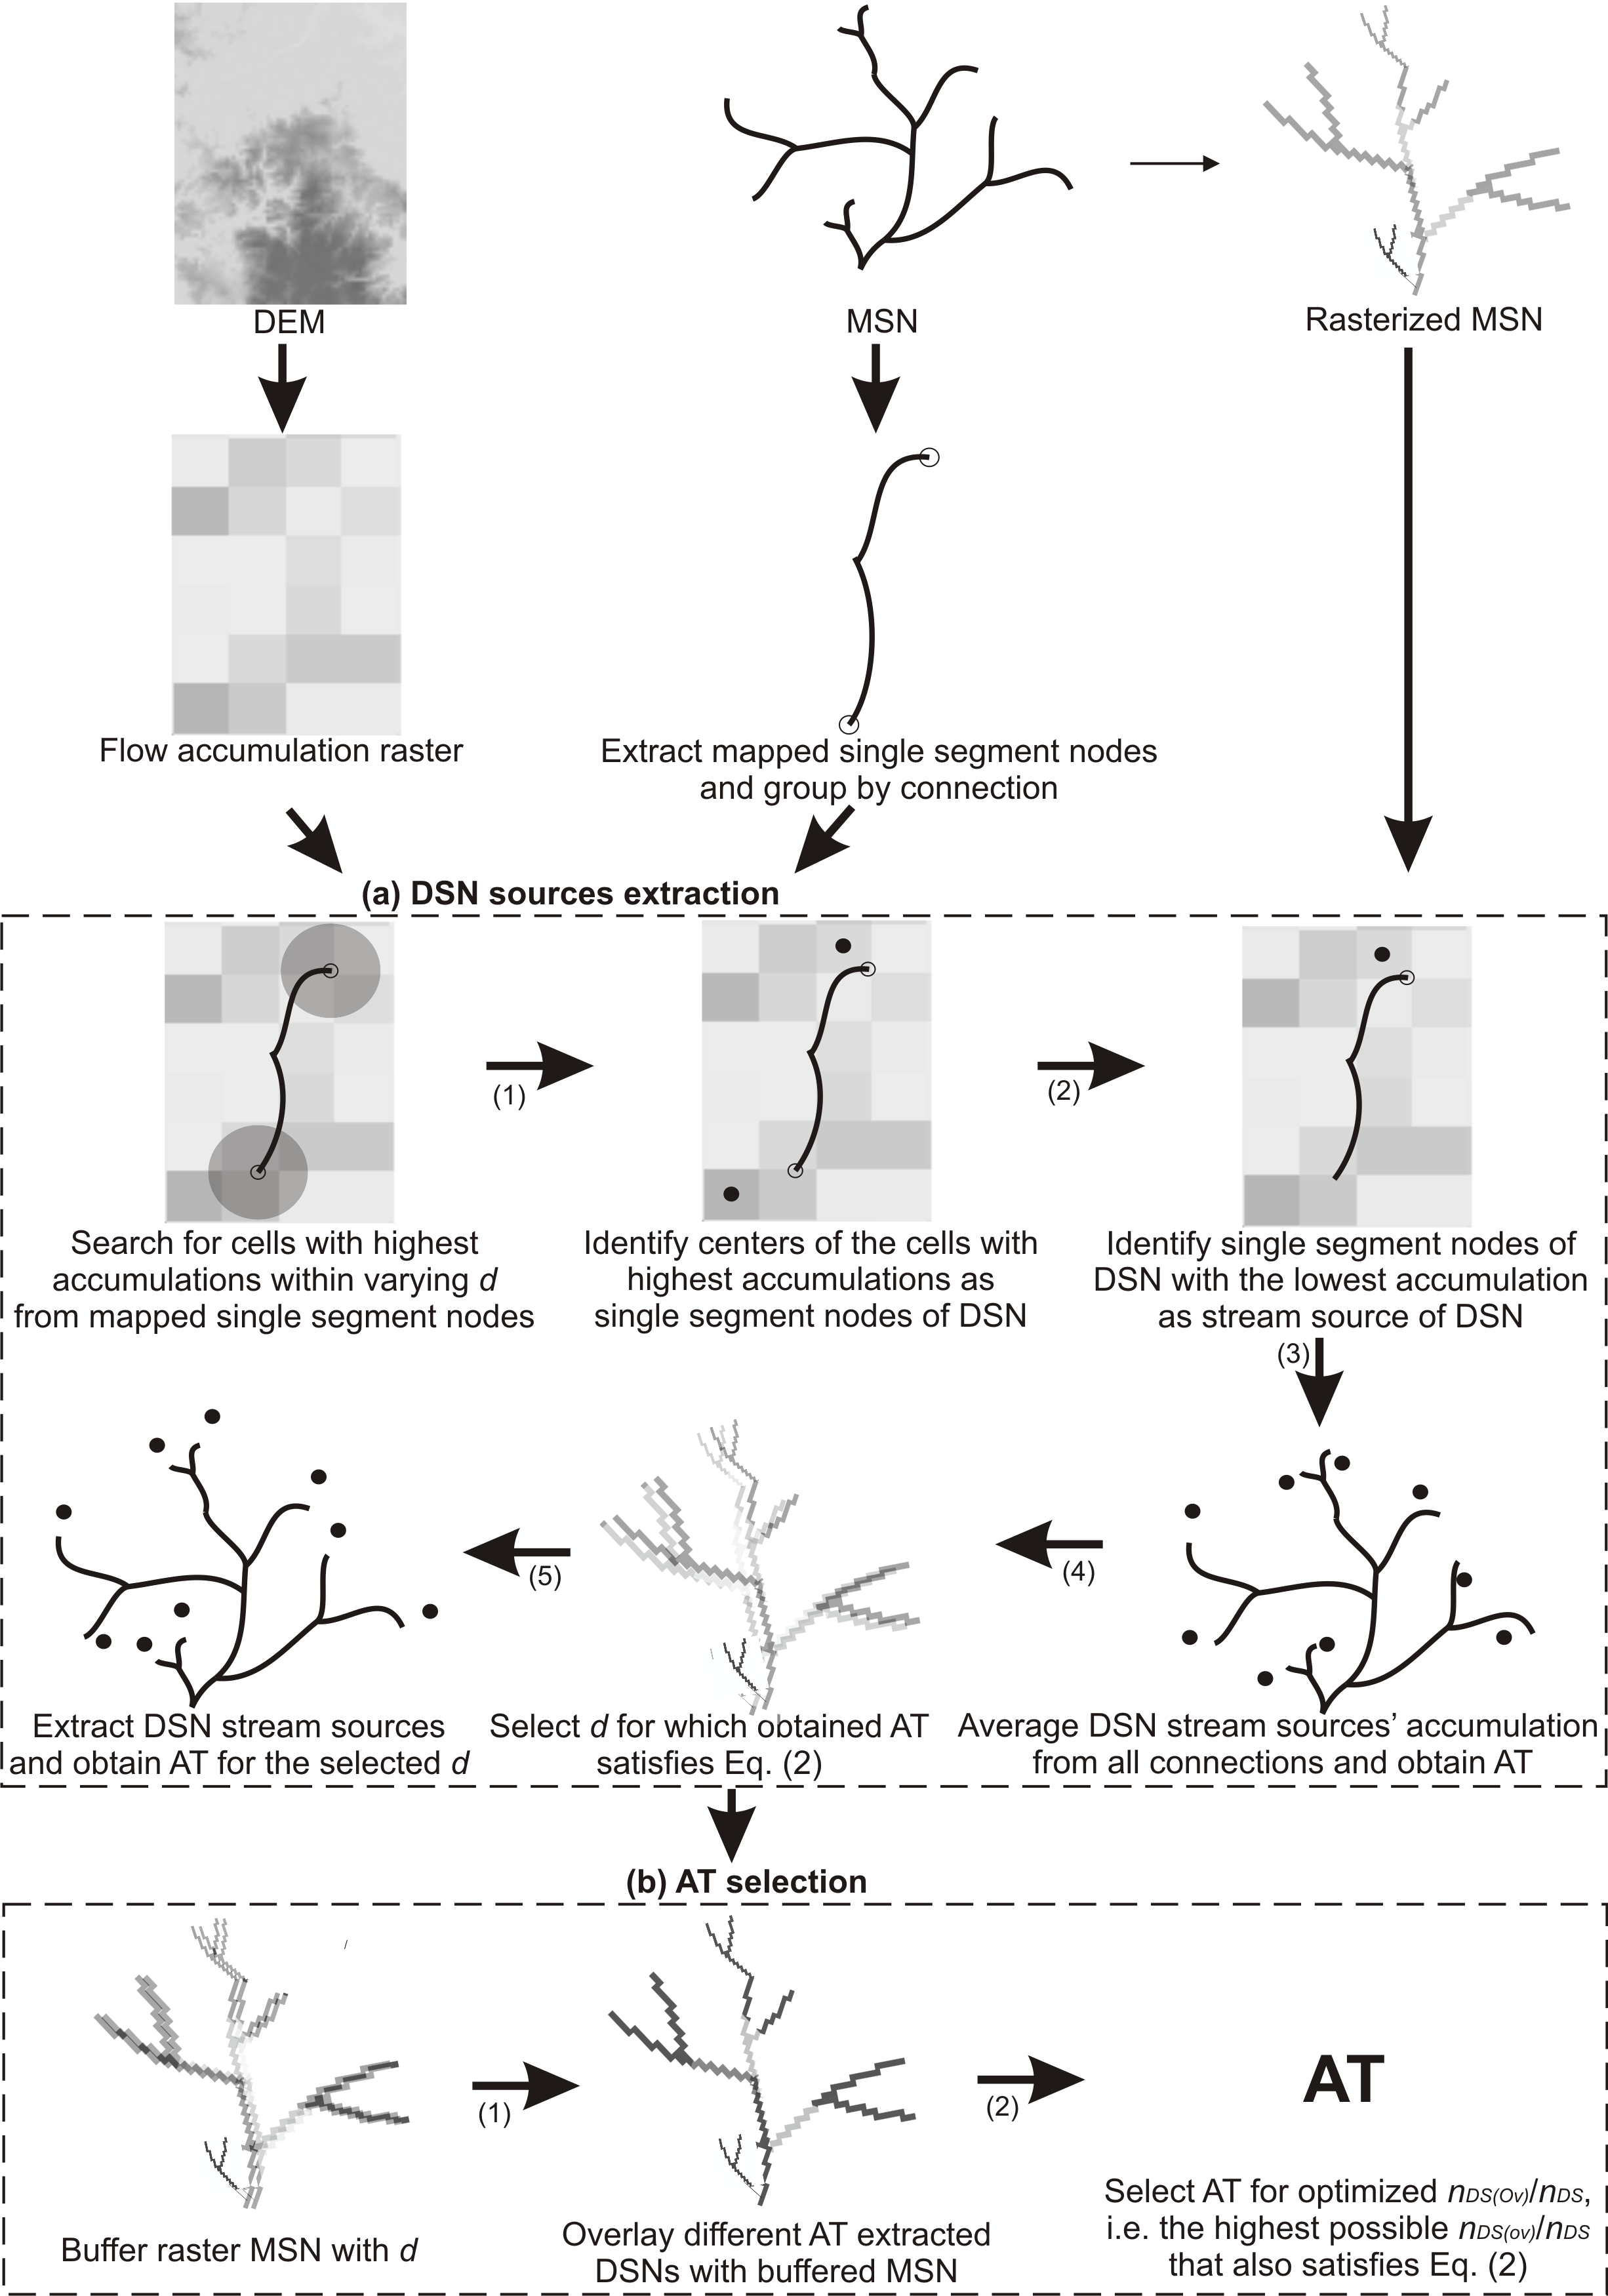
\includegraphics[width=0.8\textwidth]{Figures/Fig_2_2.png}
  \caption{The work flow of the automated accumulation threshold selection method. The used abbreviations (order: left to right and then top to bottom) – DEM: digital elevation model, MSN: mapped stream network, DSN: DEM-derived  stream network, $d$: lateral displacement between DSN and MSN, AT: accumulation threshold, $n_{DS(ov)}$: number of overlapped DEM stream cells with the selected $d$ buffered mapped stream cells and $n_{DS}$: number of DEM stream cells. The numbers below the arrows indicates the corresponding processing step.}
  \label{Fig_2_2}
\end{figure}\vspace{-0.5cm}

\item Corresponding stream sources of DSNs were identified from each group of single segment nodes of DSNs based on the lowest cell accumulations (accumulation at sources are lower than at outlets and vice versa) for the varying $d$s (see Figure 2.2(a), step 2). Then, for each $d$, an AT was computed as the mean of the accumulations at stream sources on the DEM from all groups. However, considering differences in scales and study objectives of users, the 5\textsuperscript{th}, 50\textsuperscript{th} and 95\textsuperscript{th} percentile values (can be changed by users according to their needs) of the accumulations at sources were also provided. The distributions of the AT values at stream sources of DSNs for the Hessen watershed and state Thüringen are provided in Figure A.1 in appendix A. Finally, a DSN was extracted using the AT for each of the $d$s (see Figure 2.2(a), step 3-4 and ESM A.1, 216-331).

\item The extracted number of streams ($n_{DS}$) of DSNs is an inverse function of AT, i.e. a lower AT extracts higher number of streams and vice-versa (Montgomery and Foufoula-Georgiou, 1993). Moreover, the AT increases with the width of search buffer $d$ around sources of MSNs (Figure A.2 in appendix A). Given the expected lateral displacements between the MSN and DSN, a search with a lower than optimal $d$ (Figure A.2(a)) would not include the source of the corresponding DSN and consequently yield a lower than optimal AT. By contrast, a search with a higher than optimal $d$ (Figure A.2(b)) would include non-source DSN cells and result in a higher than optimal AT. From this follows that $n_{DS}$ is an inverse function of $d$ (Eq. 2.1).

\begin{equation}
n_{DS(opt.)}=f(\frac{1}{d})
\label{Eq. 2.1}
\end{equation}

The extracted $n_{DS}$ was compared to the number of mapped stream cells ($n_{MS}$) for all $d$s and then optimized ($n_{DS(opt.)}$) by using Eq. (2).

\begin{equation}
n_{DS}=n_{MS}+min(n_{DS}-n_{MS});with\frac{n_{DS}-n_{MS}}{n_{MS}}<0.05
\label{Eq. 1.1}
\end{equation}

The term min($n_{DS} – n_{MS}$) indicates the minimum of the difference between the number of DSN and MSN stream cells. The $n_{DS}$ was constrained to be a maximum of 5\% higher than the $n_{MS}$ (as indicated by the constraints: with ($n_{DS} – n_{MS})/n_{MS}<0.05$) to assure that all streams of the MSN were extracted from the DEM and while minimizing the extraction of non-existing streams (Figure 2.2(a)).

\end{enumerate}

The $d$ that extracted $n_{DS(opt.)}$ was selected as the lateral displacement between the MSN and DSN. To increase precision, from this step $d$ was further consecutively decreased by 10 m (1/5th of the initial $d$) in the loop and the lateral displacement was selected satisfying Eq. (2). However, the initial $d$ as well as the values for the increase and decrease can be chosen by users according to their requirements regarding precision and scale of the project. The corresponding accumulation threshold for the selected lateral displacement $d$ ($AT_d$) was selected for further processing.

\subsubsection{Overlap optimization between mapped and DEM-derived streams}
\label{Overlap optimization between mapped and DEM-derived streams}

First, the mapped stream network (MSN) was buffered with the selected lateral displacement ($d$) and then overlaid with the digital elevation model (DEM)-derived stream networks (DSN) extracted for different accumulation thresholds (AT). Subsequently, the percentage of overlapped DEM-derived stream cells ($n_{DS(ov)}/n_{DS}$) was computed (see Figure 2.2(b), step 1 and ESM A.1, L 333-413). The initial AT was the one for the selected $d$ ($AT_d$) and was consecutively increased or decreased by $10^{n-1}$ unit, where $10{n-1}<AT_d\leq 10^n; n \in N$, to increase $n_{DS(ov)}/n_{DS}$. For example, the increments or decrements were 100 and 1000 for the ATds of 370 (Hessen watershed, $10<370\leq 1000$) and 8543 (Thüringen, $1000<8543\leq 10000$), respectively (see Figure 2.2(b), step 2). The highest value of the $n_{DS(ov)}/n_{DS}$ that also satisfied Eq. (2) was considered as optimal, i.e. the highest possible overlap between the MSN and DSN that also extracts all the streams of MSN from the DEM and thus minimizes non-existing streams (see Figure 2.2(b), step 2 and ESM A.1, L 333-413). To enhance precision, the optimization of AT was continued with $10^{n-2}$unit (ignored when n=1) increase or decrease until it also yielded the highest overlap that satisfied Eq. (2). The corresponding AT for the optimized $n_{DS(ov)}/n_{DS}$ was regarded as the optimal AT for comparable DSN extraction. This AT was then employed for the extraction of the DSN from previously computed flow accumulation raster (ESM A.1, L 414-417). The $n_{DS(opt.)}$ and optimized $n_{DS(ov)}/n_{DS}$  represent the goodness-of-fit measures for the DSN.

\subsection{Automated upstream riparian corridor delineation}
\label{Automated upstream riparian corridor delineation}

The automated upstream riparian corridor (URC) delineation method is outlined in Figure 2.3 and ESM A.1, L 438-590. First, upstream catchments (UC) were delineated for the given stream sampling points (SSP) (Lagacherie et al., 2010). The delineation of UCs for the original SSP data was impeded by substantial lateral displacements from mapped stream networks (MSN) (Figure A.3 in appendix A). Therefore SSPs were first snapped to the  MSN by matching their corresponding stream names (see Figure 2.3(a), step 1). Nonetheless, users may also snap SSP to MSN by shortest euclidean distance if stream names are not available . Thereafter, previously snapped SSPs were snapped to the approximate DSN by shortest euclidean distance. If the DSN is extracted without comparing to a MSN (integration with other tools for automated AT extraction (Montgomery and Foufoula-Georgiou, 1993; Tarboton, 2005) or no MSN is available), the SSPs could be directly snapped to the DSN by shortest euclidean distance, as suggested by (Tarboton, 2005).

The length and width of the URCs were set to 10 km and 100 m, respectively, as these parameters are frequently used in freshwater research (though can be changed by users according to their study objectives) (Lorenz and Feld, 2013). However, the algorithm could also be integrated with other tools for delineating riparian corridors based on geomorphology and stream side characteristics (Abood et al., 2012; Fernández et al., 2012; Holmes and Goebel, 2011), allowing for the delineation of URCs of variable lengths and widths. Stream sections of the defined length were extracted from all stream segments that were connected to SSPs as upstream segments were unknown. This also included extracting junctions and bifurcations of stream sections. These stream sections were buffered by the defined width (see Figure 2.3(b), step 1). Then the buffered stream sections were masked by the previously extracted UCs yielding to the final URCs (see Figure 2.3(b), step 2 and ESM A.1, L 532-579). In case of integration with other tools, delineated riparian corridors for stream and stream sections by those tools need to be masked by the UCs to delineate URCs of variable sizes for given SSPs.

The complete R script for the analyses that is provided as the electronic supplementary materials (ESM) A.1 contains detailed commentary on each step. To allow for reproducibility, the required DEM, MSN and SSP data are also made available in an online repository:

\noindent \href{http://doi.pangaea.de/10.1594/PANGAEA.825001}{http://doi.pangaea.de/10.1594/PANGAEA.825001}.

\subsection{Comparison with other algorithms}
\label{Comparison with other algorithms}

ATRIC was compared with the available two algorithms (Heine et al., 2004; Lin et al., 2006) that automated the accumulation threshold (AT) selection process through a similar approach, i.e. comparison with mapped stream networks (MSN). The equivalent goodness-of-fit measures for the digital elevation model (DEM)-derived stream networks (DSN), i.e. percentage of “error stream length” in Heine et al. (2004) and “overlaid coincidental stream links” in Lin et al. (2006), were obtained and adjusted, i.e. “100-percentage of error stream length” for Heine et al. (2004). Hereafter, these measures were compared to the goodness-of-fit measure of ATRIC, i.e. percentage of overlapped stream cells with buffered mapped streams ($n_{DS(ov)}/n_{DS}$). Simultaneously, the corresponding spatial scales (extents) of the study areas were also compared.

\section{Results and Discussion}
\label{Results and Discussion}

\subsection{Automated accumulation threshold and spatial scale}
\label{Automated accumulation threshold and spatial scale}

In this paper, we developed ATRIC that extracted stream networks (DSN) from digital elevation

\noindent\begin{figure}[h!]
  \centering
  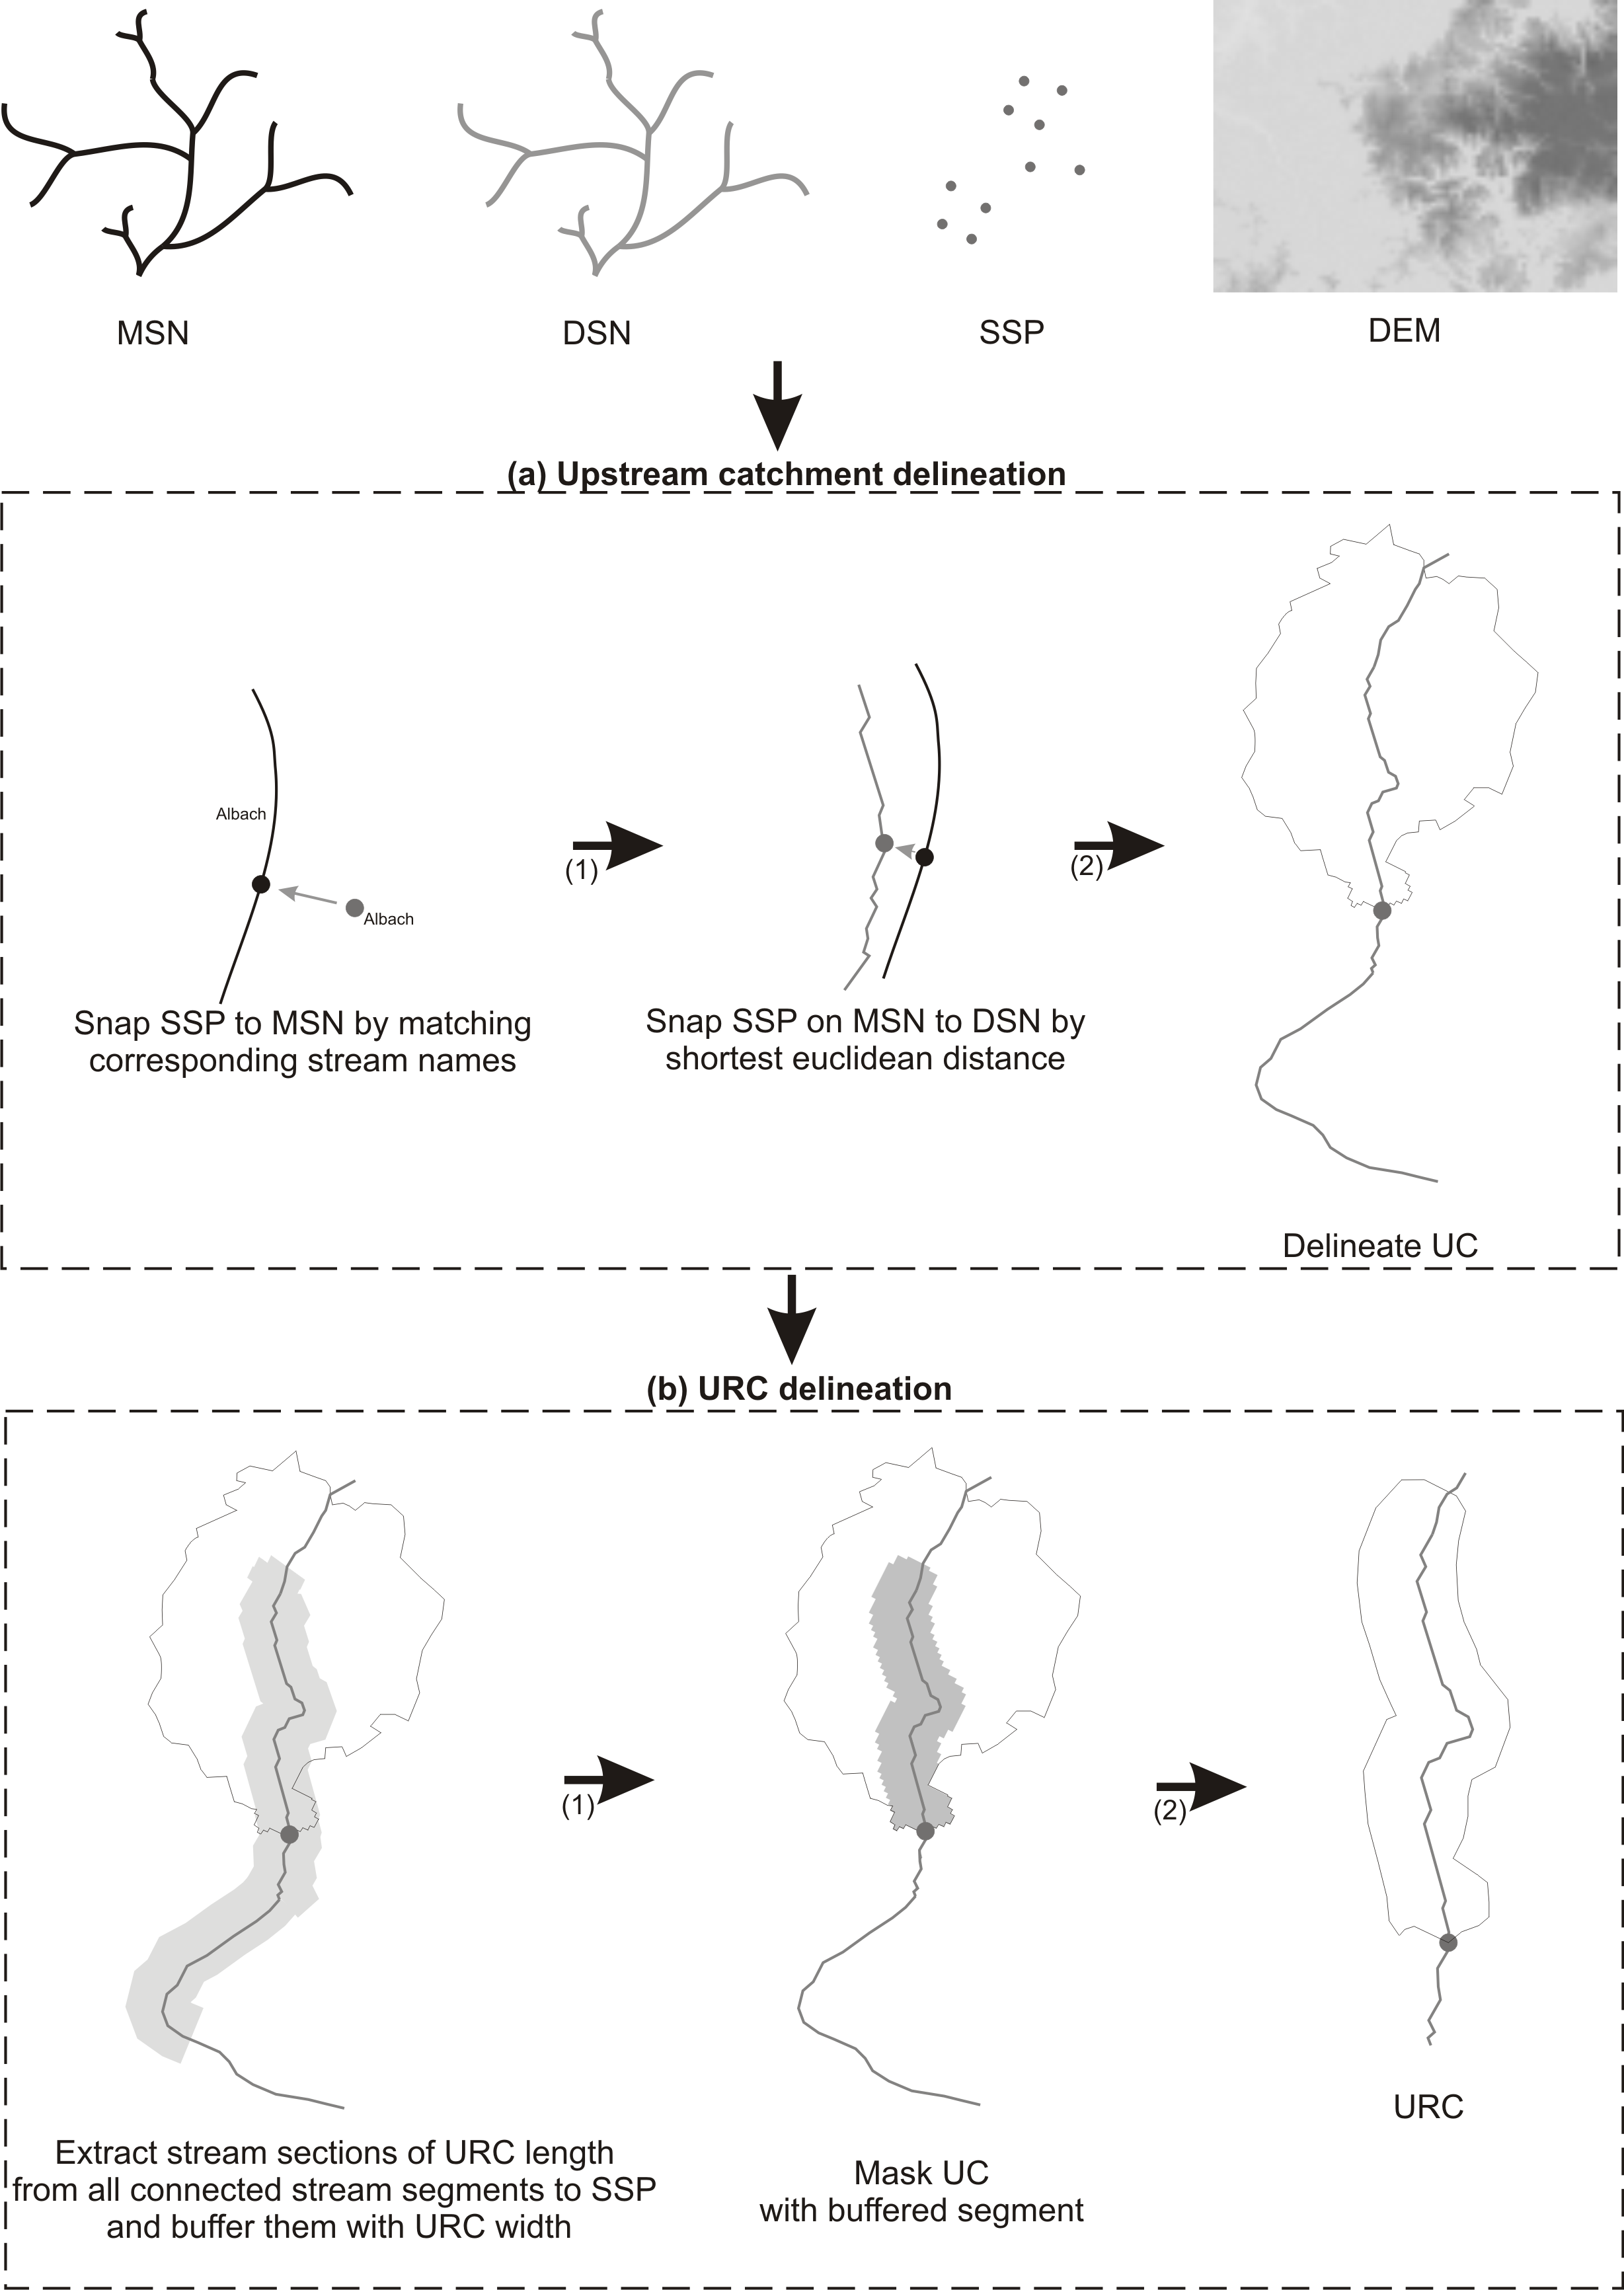
\includegraphics[width=0.8\textwidth]{Figures/Fig_2_3.png}
  \caption{The work flow of the upstream riparian corridor delineation method for given stream sampling points. The used abbreviations (order: left to right and then top to bottom) – MSN: mapped stream network, DSN: digital elevation model (DEM)-derived stream network,  SSP: stream sampling points and URC: upstream riparian corridor. The numbers below the arrows indicates the corresponding processing step.}
  \label{Fig_2_3}
\end{figure}

\noindent models (DEM) using automatically selected accumulation thresholds (AT) that maximize concordance with traditionally mapped stream networks (MSN). The tool was applied on two different spatial scales (extents), given that spatial scale impacts on the selection of an AT (Murphy et al., 2008). Large scale studies require DSNs of high stream orders, e.g. in large watersheds, corresponding to the selection of a high AT. Conversely, small scale studies often focus on lower stream order and dense DSNs corresponding to the selection of a low AT. However, ATRIC automatically adjusts to the scale of the provided MSNs and selects an AT on the related scale conditional that the resolution of the used DEMs is appropriate. For example, a small scale study that requires a dense stream network should apply DEM with a sufficiently high resolution, whereas a coarse-resolution DEM might suffice for a large scale study. Overall, users of ATRIC should select DEMs with appropriate resolution with respect to the order and density of MSNs.

\subsection{Goodness of stream network extraction from digital elevation models}
\label{Goodness of stream network extraction from digital elevation models}

The digital elevation model (DEM)-derived stream networks (DSN) extracted by ATRIC exhibited good agreement with the mapped stream networks (MSN) on both spatial scales (Table 2.1 and 2.2; Figure 2.4). The AT obtained from the automatically selected $d$ ($AT_d$, 370 and 8543) for the Hessen watershed and state Thüringen extracted almost equivalent (2.93\% and 4.77\% higher) number of DSN ($n_{DS}$) compared to the number of MSN stream cells ($n_{MS}$) (Table 2.1). The ATs (500 and 9543) obtained from the further optimization of the $AT_d$s were marginally different from the $AT_d$s but considerably improved the concordance between the $n_{DS}$ and $n_{MS}$, i.e. obtained $n_{DS}$s were only 0.24\% and 0.43\% higher than the $n_{MS}$s for the Hessen watershed and state Thüringen, respectively (Table 2.2). Moreover, the extracted DSNs entailed high (89.36\%) and moderate (57.42\%) overlaps with the MSNs buffered with the selected $d$s for the Hessen watershed and state Thüringen, respectively (Table 2.2).

When compared to the goodness-of-fit of other algorithms on comparative spatial scales, ATRIC showed similar or better performance (Table 2.3). The spatial extent of the Hessen watershed is 75 times larger and 1.6 times smaller on average than the watersheds used in Heine et al. (2004) and Lin et al. (2006), respectively. Nevertheless, while compared to Heine et al. (2004) and Lin et al. (2006), the goodness-of-fit of the extracted DSN for the Hessen watershed was higher. However, the goodness-of-fit of the extracted DSN for the state Thüringen was lower where the spatial extent

\noindent\begin{table}[h!]
\label{Table 2.1}
\caption{The results of number of digital elevation model (DEM)-derived stream cells ($n_{DS}$) optimization to obtain average lateral displacements ($d$) between mapped stream network (MSN) and DEM-derived stream network (DSN). The computed accumulation threshold (AT), $n_{DS}$ and the percentage high or low are the $n_{DS}$ from the number of mapped stream cells ($n_{MS}$), i.e. (($n_{DS}-n_{MS})/n_{MS}$) are reported with varying $d$s.}
\begin{threeparttable}
\centering
\begin{tabular}{>{\centering\arraybackslash}m{2.6cm}>{\centering\arraybackslash}m{1.5cm}>{\centering\arraybackslash}m{3cm}>{\centering\arraybackslash}m{2.5cm}>{\centering\arraybackslash}m{0.7cm}>{\centering\arraybackslash}m{1.3cm}}

\toprule
\textbf{Spatial scale} & \textbf{Variable $d$} & \textbf{Consecutive increase or decrease in the $d$} & \textbf{Computed AT} & \textbf{$n_{DS}$} & \textbf{$\frac{n_{DS} - n_{MS}}{n_{MS}}$}\\
 & \textbf{$(m)$} & \textbf{$(+/- m)$} & & & \textbf{$(+/- \%)$}\\

\midrule

 & 50 & - & 55 & 3469 & +182.49\\
 & 100 & +50 & 263 & 1734 & +41.21\\
 & 150 & +50 & 362 & 1325 & +7.89\\
Hessen watershed & 200 & +50 & 654 & 1086 & -11.56\\
 & 190 & -10 & 652 & 1088 & -7.00\\
 & 180 & -10 & 592 & 1142 & -7.00\\
 & 170 & -10 & 572 & 1167 & -4.97\\
 &
 \rowcolor{Gray}
 160 & -10 & 370 & 1264 & +2.93\\
\hline
 & 50 & - & 279 & 986647 & +391.92\\
 & 100 & +50 & 1717 & 442971 & +120.85\\
Thüringen state & 150 & +50 & 9756 & 199451 & -0.56\\
 &
 \rowcolor{Gray}
 140 & -10 & 8543 & 210133 & +4.77\\
 & 130 & -10 & 8485 & 212799 & +6.09\\

\bottomrule

\end{tabular}
\begin{tablenotes}
\footnotesize
\colorbox{Gray}{Grey highlighted} = The obtained $d$ between $DSN$ and $MSN$ by $n_{DS}$ optimization, corresponding $AT (AT_d)$ and $\frac{n_{DS} – n_{MS}}{n_{MS}}$ 
\end{tablenotes}
\end{threeparttable}
\end{table}

\newpage

\noindent\begin{table}[t!]
\label{Table 2.2}
\caption{The results of overlapped digital elevation model (DEM)-derived stream cells ($n_{DS(ov)}$) with buffered mapped stream cells optimization to select an accumulation threshold (AT). The percentages of overlapped DEM-derived stream cells ($n_{DS(ov)}/n_{DS}$) with varying ATs are reported.}
\centering
\begin{threeparttable}
\begin{tabular}{>{\centering\arraybackslash}m{2.6cm}>{\centering\arraybackslash}m{1.5cm}>{\centering\arraybackslash}m{4cm}>{\centering\arraybackslash}m{1.5cm}>{\centering\arraybackslash}m{1.5cm}}

\toprule
\textbf{Spatial scale} & \textbf{AT} & \textbf{Consecutive increase or decrease in the AT starting from the $AT_d$ (Table 2.1)} & $\frac{n_{DS}(ov)}{n_{DS}}$ & $\frac{n_{DS} - n_{MS}}{n_{MS}}$\\
 & & $+/- unit$ & $(\%)$ & (+/- \%)\\

\midrule

 & 370 & - & 83.15 & +2.93\\
 & 470 & +100 & 88.53 & +2.06\\
 Hessen watershed & 480 & +10 & 88.90 & +1.22\\
 & 490 & +10 & 89.32 & +0.65\\
 &
 \rowcolor{Gray}
 500 & +10 & 89.36 & +0.24\\
 & 510 & +10 & 90.06 & -0.90\\
\hline
 & 8593 & - & 56.06 & +4.77\\
Thüringen state &
\rowcolor{Gray}
9543 & +1000 & 57.42 & +0.43\\
 & 9643 & +100 & 57.53 & -0.04\\
 
\bottomrule

\end{tabular}
\begin{tablenotes}
\footnotesize
\colorbox{Gray}{Grey highlighted} = The AT obtained by $n_{DS}(ov)/n_{DS}$ optimization and corresponding $\frac{n_{DS}(ov)}{n_{DS}}$ and $\frac{n_{DS} - n_{MS}}{n_{MS}}$
\end{tablenotes}
\end{threeparttable}
\end{table}

\vspace{-1.0cm}\noindent\begin{table}[h!]
\label{Table 2.3}
\caption{Comparison of the goodness-of-fit of the ATRIC extracted stream networks from the digital elevation models (DEM) with the stream networks extracted by other algorithms for automated accumulation threshold selection.}
\centering
\begin{tabular}{>{\centering\arraybackslash}m{1.5cm}>{\centering\arraybackslash}m{2.2cm}>{\centering\arraybackslash}m{1.5cm}>{\centering\arraybackslash}m{1.8cm}>{\centering\arraybackslash}m{3.5cm}>{\centering\arraybackslash}m{1.5cm}}

\toprule
\textbf{Source} & \textbf{Study area} & \textbf{Spatial extent} & \textbf{Resolution of the used DEMs} & \textbf{Comparable measure of the goodness-of-fit} & \textbf{Goodness-of-fit}\\
 & & $km^2$ & $(m)$ & & $(\%)$\\

\midrule

 Heine et al. (2004) & Tallgrass National Park watershed & 0.6 & 10 & 100 – percentage of total error stream & 87.30\\
 \hline
 \multirow{2}{1.5cm}{\centering Lin et al.(2006)} & Chi-Jia-Wang watershed & 74.03 & \multirow{2}{1.5cm}{\centering 40} & \multirow{2}{3.5cm}{\centering Percentage of overlaid coincidental stream links} & 70\\
 & Erh-Wu watershed & 51.36 & & & 72\\
 \hline
 \multirow{2}{*}{\centering ATRIC} & Hessen watershed & 45 & \multirow{2}{1.5cm}{\centering 25} & \multirow{2}{3.5cm}{\centering Percentage of overlapped stream cells with mapped streams buffered by a selected lateral displacement} & \vspace{12pt} 89.36\\[0.6cm]
 & Thüringen state & 16171 & & & \vspace{12pt} 57.42\\[0.6cm]
 
\bottomrule

\end{tabular}
\end{table}

\noindent was approximately 360 times larger than the Hessen watershed. These results are supported by Goodchild and Gopal (1989) and Murphy et al. (2008), who showed that the goodness-of-fit of GIS analyses is scale-dependent, e.g. smaller scale stream extraction results in better goodness-of-fit. Moreover, constant ATs selected on smaller spatial scales are more representative of the topography and geomorphology of study areas because of more homogeneity and hence, yield better overlap with MSNs (Heine et al., 2004; Lin et al., 2006). However, ATRIC represents an improvement in extraction precision on large scales because of optimization of the $n_{DS}$ before determining the $n_{DS(ov)}/n_{DS}$ and thus advances previous algorithms.

\noindent\begin{figure}[h!]
  \centering
  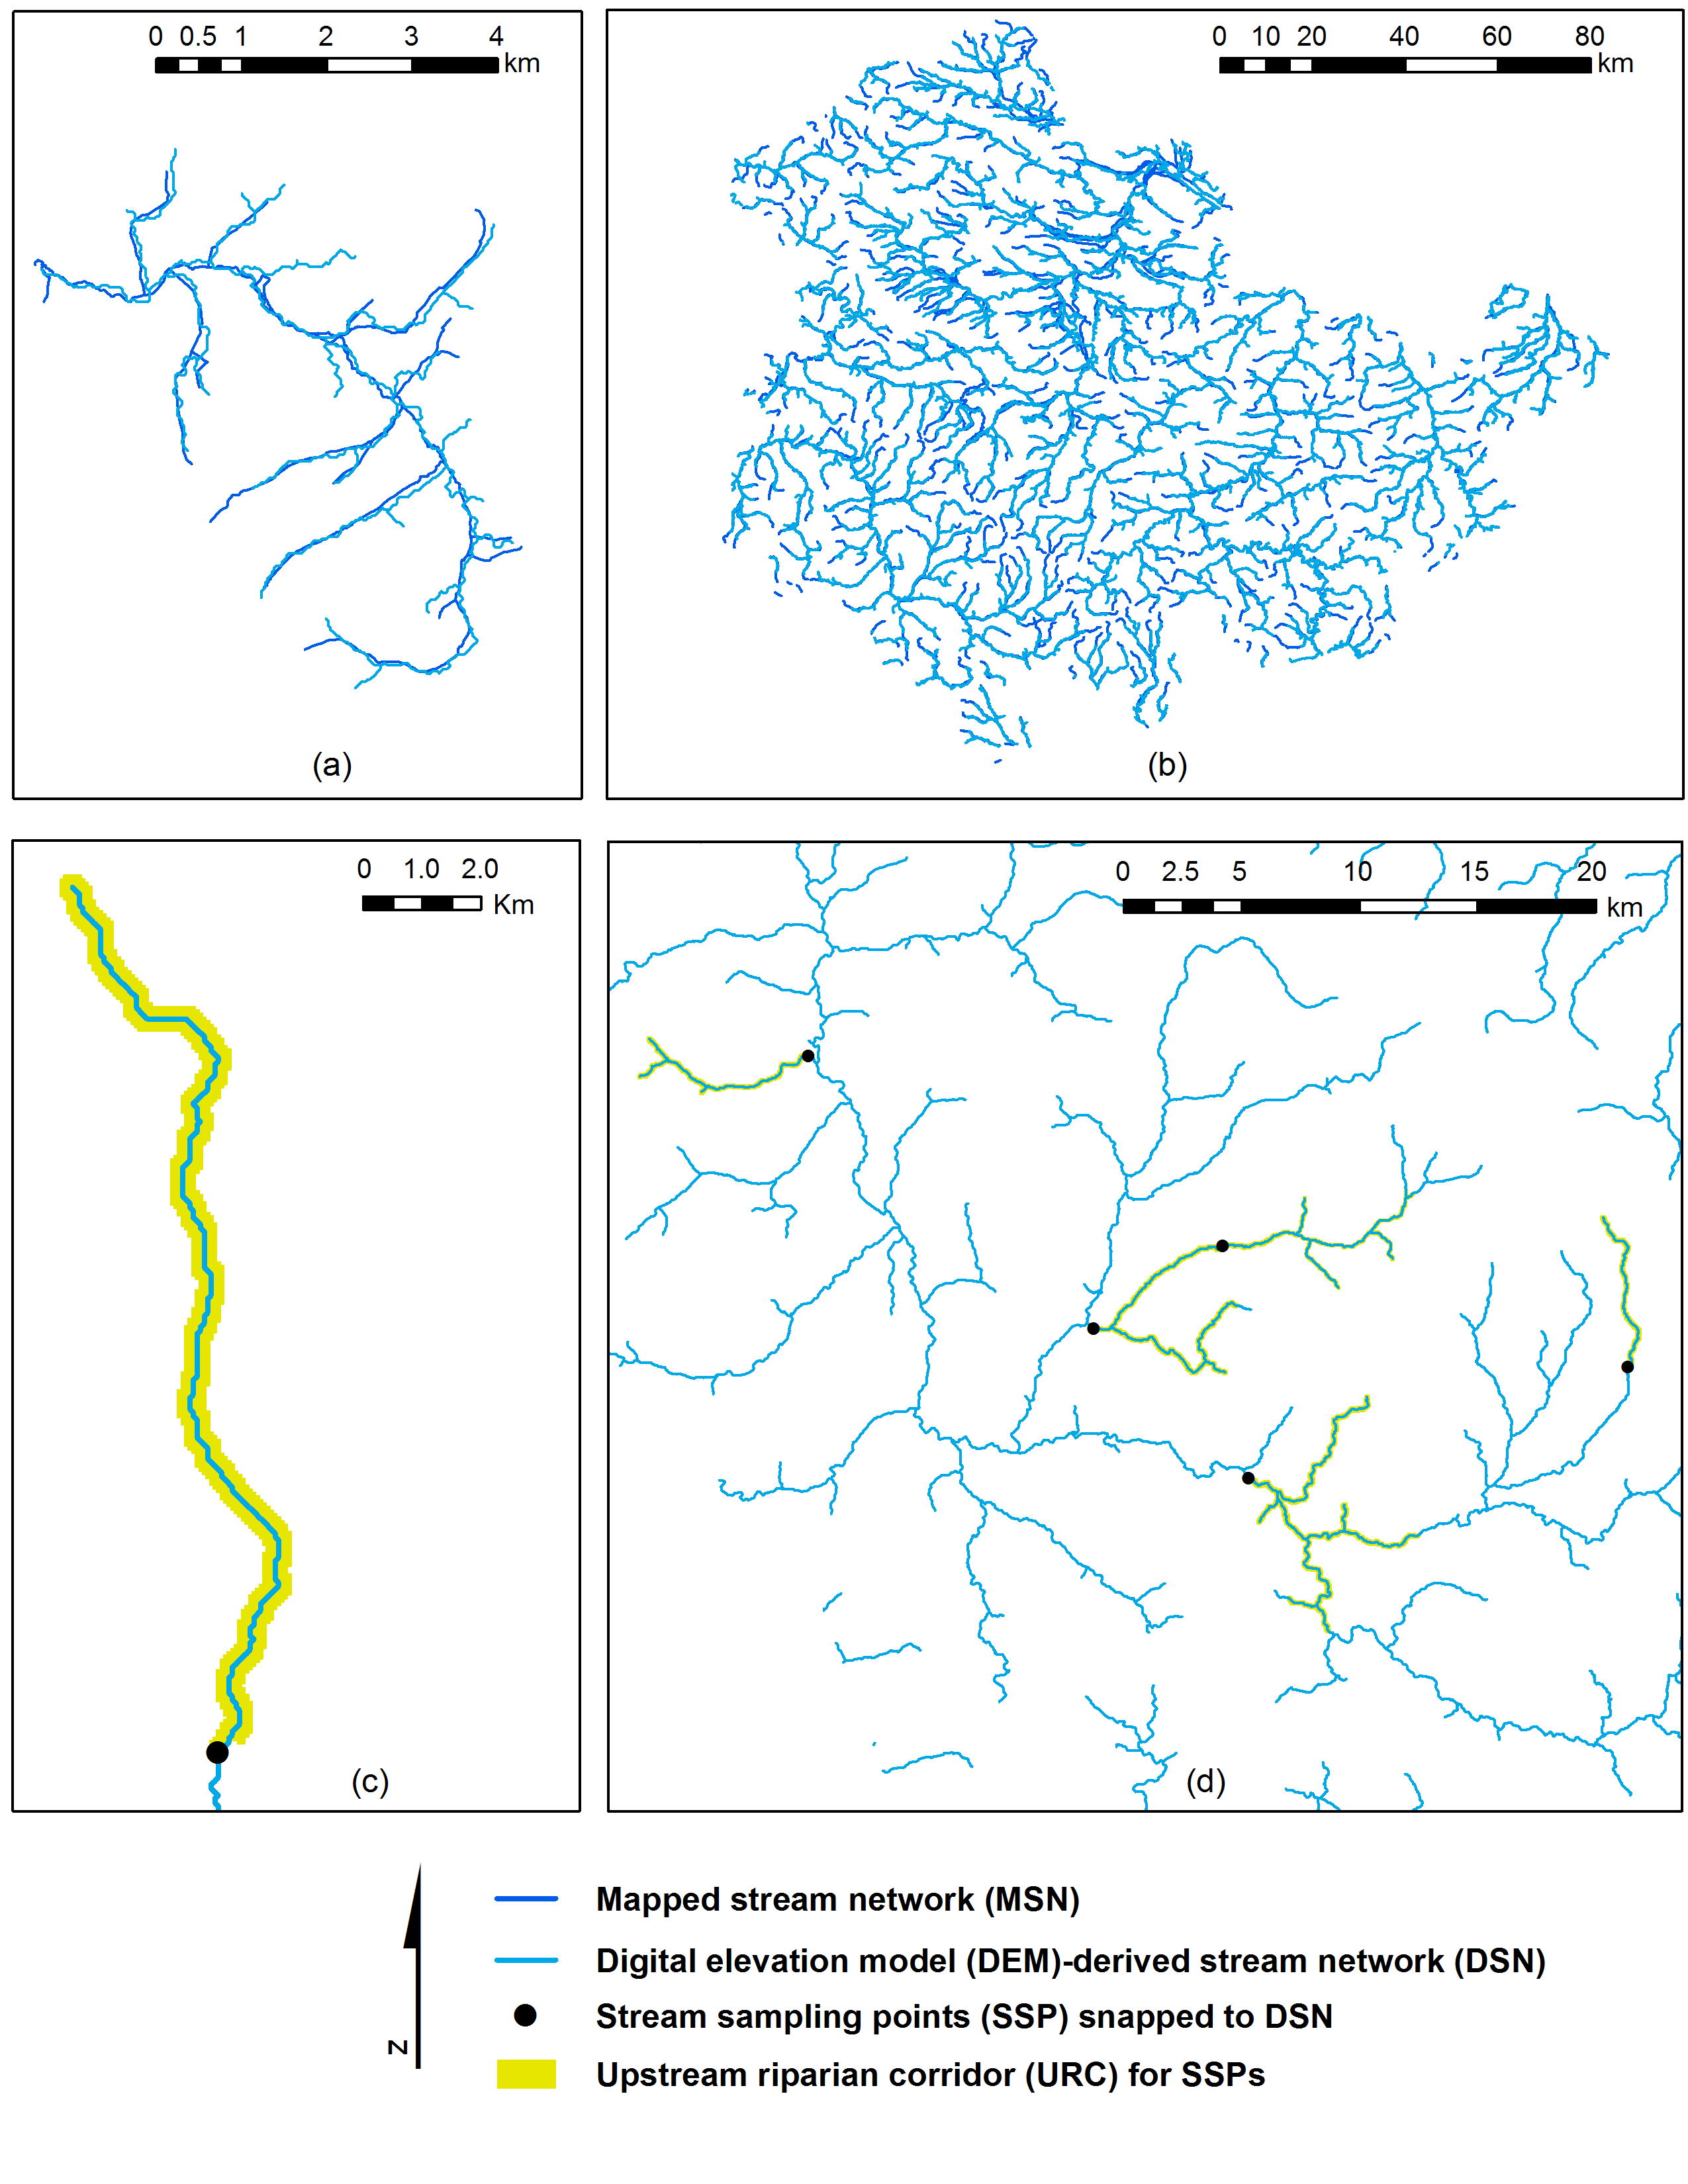
\includegraphics[width=0.785\textwidth]{Figures/Fig_2_4.png}
  \caption{The digital elevation model (DEM)-derived stream networks (DSN) by ATRIC overlaid with mapped stream networks (MSN) in (a) the watershed at the northeast of Hessen and (b) Thüringen, and delineated upstream riparain corridors (URC) of (c) one stream sampling point (SSP) in the Hessen watershed and ($d$) several SSPs in Thüringen.}
  \label{Fig_2_4}
\end{figure}

Geographic characteristics of study regions also influence the goodness of DSN (Wolock et al., 1990). The study regions reported in Heine et al. (2004) and Lin et al. (2006) were flat, simple and homogeneous whereas we applied ATRIC on relatively complex and heterogeneous regions and obtained comparable goodness of DSN.

Resolution, sources and creation methods of DEM also substantially affect the goodness of DSN (Li and Wong, 2010; McMaster, 2002; Murphy et al., 2008). Therefore goodness of ATRIC can be further improved by using a higher resolution (e.g. 10 m) and more advanced equipment derived (e.g. lidar) DEMs.

\clearpage

\vspace{-1.1cm}

\subsection{Computational efficiency}
\label{Computational efficiency}

ATRIC showed high computational efficiency in terms of required computation time and size of input datasets. We ran ATRIC on three different computers: (1) Linux OS with 3.8 GHz Quad-Core processor and 16 GB RAM, (2) Mac OS with 2.8 GHz Quad-Core processor and 12 GB RAM and (3) Windows OS with 2.9 GHz Dual-Core processor and 4 GB RAM. Required time for automated accumulation threshold (AT) selection on the small (watershed) and large (state) spatial scales on the Linux, Mac, Windows OS computers were 43 seconds, 58 seconds, two minutes and 33 minutes, 50 minutes, two hours, respectively. The time required for the upstream riparian corridor (URC) delineation per stream sampling point (SSP) was 30 seconds for Linux and Mac OS, and one minute for Windows OS, respectively. Moreover, the other available algorithms for automated AT selection (Heine et al., 2004; Lin et al., 2006; Montgomery and Foufoula-Georgiou, 1993; Tarboton, 2005) were developed on single watersheds and therefore the input digital elevation models (DEM) and mapped stream networks (MSN) that were processed were small in terms of number of cell. By contrast, ATRIC processed large input DEM and MSN in the state Thüringen that is comprised of 100 watersheds and a complex topography. Thus ATRIC showed an advantage over the available algorithms in terms of processing large datasets. This computational efficiency was entailed by the efficient raster processing capability in R and GRASS GIS (GRASS Development Team, 2014; R Core Team, 2014).

\vspace{-0.25cm}

\subsection{Development and integration}
\label{Development and integration}

ATRIC is the first algorithm that has been developed using free and open source software. The available algorithms relying on proprietary software have already shown substantial improvement in stream network mapping (Heine et al., 2004; Lin et al., 2006). Given the rapid growth in the market shares of open source GIS software packages (Neteler et al., 2012), ATRIC enables widespread usage and thus improvement in stream network mapping. Moreover, non-profit community motivation, non-proprietary hierarchical co-ordination and coherence with proprietary standards of the open source software ensure further development of ATRIC (Bonaccorsi and Rossi, 2003).

ATRIC was developed combining two different software packages (R and GRASS GIS) and thus advanced available GIS operations (Bivand, 2007). R provides platforms for co-interfacing with several other free open source (e.g. “SAGA GIS” (Brenning, 2007) by the package “RSAGA” (Brenning, 2008)) and proprietary (e.g. ArcGIS (ESRI, Redlands, 2001) by the package “RPyGeo” (Brenning, 2012)) GIS software packages. Thus ATRIC could be further integrated with other GIS software  packages. Importantly, ATRIC will facilitate the reproducibility of geoscientific research (Pebesma et al., 2012).

Moreover, ATRIC can be integrated with other algorithms for statistical and geostatistical modeling on stream network, i.e. SSN (Ver Hoef et al., 2012) and rtop (Skøien et al., 2014), and extraction of riparian corridors for streams and stream sections based on streamside characteristics and geomorphological analyses (Abood et al., 2012; Fernández et al., 2012; Holmes and Goebel, 2011). Currently, the data required for SSN is provided by STARS (Peterson and Ver Hoef, 2014) that depends on ArcGIS (proprietary software). ATRIC represents an open source alternative because it includes tools for building network topology, extracting a comparable digital elevation model (DEM)-derived stream network (DSN) for a given mapped stream network (MSN) considering the lateral displacement (instead of burning the MSN into the DEM which is done in STARS) and upstream catchment (UC) delineation for given points on streams. Delineating UC for given stream sampling points on MSN is also a primary requirement in rtop. Moreover, ATRIC can be integrated to extract upstream geomorpholocial riparian corridors of variable sizes for particular stream sampling points (SSP).

\vspace{-0.25cm}

\subsection{Potential fields of application}
\label{Potential fields of application}

Advances in computer technology and GIS software, and widespread availability of electronic maps and high resolution satellite imagery in recent decades facilitate far reaching applications for ATRIC. These include related fields of freshwater research, e.g. cartography, geomorphology, hydrology, ecology and water resources management. Some examples are:

\begin{enumerate}[(i)]

\item Improving accuracy, precision and efficiency of digital and traditional topographic mapping by providing high quality digital elevation model (DEM)-derived stream network (DSN, hydrological) data layers (Heine et al., 2004),

\item Enabling geomorphological analyses, e.g. flood modeling on DEM by providing corresponding DSN as such analyses are not possible on areal photographs or traditional paper maps (Gichamo et al., 2012),

\item Updating existing stream network maps by frequently updated and easily available DEMs (Olivera, 2001),

\item Extracting stream networks in unmapped regions (traditionally mapped stream networks (MSN) are not available) using the accumulation threshold (AT) derived from mapped regions (MSN available) by ATRIC. This is applicable when the unmapped region has an identical size and topography as well as environmental characteristics of the mapped region and the scales of the studies on two regions are the same. Moreover, as AT is assumed to correlate with different regional geomorphological and climatological parameters, such as plane curvature and precipitation  (Moore et al., 1991), the AT for unmapped regions could also be predicted based on the relationship of ATs in several mapped regions with these regional parameters, and

\item Detecting and quantifying different stressors due to landuse and climate change, surface runoff, ingredient flow in the URCs for convergent SSPs (Lorenz and Feld, 2013).

\end{enumerate}

Moreover, ATRIC overcame the problem of lateral displacements between MSN and DSN and can extract DSN sources without DEM alteration. Hence, ATRIC can be applied across different DEM with variable resolution, accuracy and precision for DSN extraction and URC delineation.

\section{Conclusions and outlook}
\label{Conclusions and outlook}

We developed ATRIC for the automation of accumulation threshold (AT) selection to enable objective stream network extraction and upstream riparian corridor (URC) delineation from digital elevation models (DEM) using open source software packages. The DEM-derived stream networks (DSN) by ATRIC represented a good approximation of the given mapped stream network (MSN). However, traditional field survey and derived MSNs often miss important stream stretches (Colson et al., 2008). This might affect the goodness of the extracted DSN when compared to ground truth as ATRIC primarily depends on the provided mapped stream cells. It might also affect reliability of the delineated URC for a given set of stream sampling points (SSP) because this delineation depends on the extracted approximate DSN. Nevertheless, the MSN provided by governmental authorities are widely accepted as the most accurate and precise ground truth. Moreover, the MSNs used here were previously validated against digital landscape models and orthophotos and hence, can be claimed to be less erroneous. In contrast to previous approaches (e.g. Heine et al. (2004) and Lin et al. (2006)), ATRIC is relatively independent of the location of mapped stream sources in AT selection and thus stream network extraction. Notwithstanding, future studies could enhance ATRIC by integrating variable AT selection in case of a complex topography. Furthermore, if high resolution satellite imageries are available, the DSN could be validated using satellite imageries in case that the provided MSN is erroneous. Finally, implementation of ATRIC as a pure GIS module, e.g. GIS package in R or GRASS GIS toolkit, to avoid co-interfacing as well as development of a graphical user interface might enhance accessibility and migration to other GIS platforms.

\openleft

\begingroup

\renewcommand{\addcontentsline}[3]{}

\begin{thebibliography}

\bibitem{} \hangindent=1cm Abood, S.A., Maclean, A.L., Mason, L.A., 2012. Modeling Riparian Zones Utilizing DEMS and Flood Height Data. Photogrammetric engineering and remote sensing 78, 259–269.

\bibitem{} \hangindent=1cm Arge, L., Chase, J.S., Halpin, P., Toma, L., Vitter, J.S., Urban, D., Wickremesinghe, R., 2003. Efficient flow computation on massive grid terrain datasets. GeoInformatica 7, 283–313.

\bibitem{} \hangindent=1cm Bastian, C.T., McLeod, D.M., Germino, M.J., Reiners, W.A., Blasko, B.J., 2002. Environmental amenities and agricultural land values: a hedonic model using geographic information systems data. Ecological Economics 40, 337–349.

\bibitem{} \hangindent=1cm Berhane, G., Walraevens, K., 2013. Geological and geotechnical constraints for urban planning and natural environment protection: a case study from Mekelle City, Northern Ethiopia. Environmental Earth Sciences 69, 783–798. doi:10.1007/s12665-012-1963-x

\bibitem{} \hangindent=1cm Biss, R., Kübler, P., Pinter, I., Braukmann, U., 2006. Leitbildbezogenes biozönotisches Bewertungsverfahren für Fließgewässer in der Bundesrepublik Deutschland -Ein erster Beitrag zur integrierten ökologischen Fließgewässerbewertung (Project report No. 298 24 777), UBA-FB 000348. Umweltforschungsplan des Bundesministeriums für Umwelt, Naturschutz und Reaktorsicherheit, Berlin.

\bibitem{} \hangindent=1cm Bivand, R., 2007. Using the R–Grass interface. OSGeo Journal 1, 36–38.

\bibitem{} \hangindent=1cm Bivand, R., Rundel, C., 2012. rgeos: Interface to Geometry Engine-Open Source (GEOS). R package version 0.2-2.

\bibitem{} \hangindent=1cm Bonaccorsi, A., Rossi, C., 2003. Why Open Source software can succeed. Research Policy 32, 1243–1258. doi:10.1016/S0048-7333(03)00051-9.

\bibitem{} \hangindent=1cm Brenning, A., 2007. RSAGA: SAGA geoprocessing and terrain analysis in R.

\bibitem{} \hangindent=1cm Brenning, A., 2012. RPyGeo: ArcGIS geoprocessing in R via Python.

\bibitem{} \hangindent=1cm Callow, J.N., Van Niel, K.P., Boggs, G.S., 2007. How does modifying a DEM to reflect known hydrology affect subsequent terrain analysis? Journal of Hydrology 332, 30–39. doi:10.1016/j.jhydrol.2006.06.020.

\bibitem{} \hangindent=1cm Colson, T., Gregory, J., Dorney, J., Russell, P., 2008. Topographic and soil maps do not accurately depict headwater stream networks. National Wetlands Newsletter 30, 25–28.

\bibitem{} \hangindent=1cm Dahm, V., Hering, D., Nemitz, D., Graf, W., Schmidt-Kloiber, A., Leitner, P., Melcher, A., Feld, C.K., 2013. Effects of physico-chemistry, land use and hydromorphology on three riverine organism groups: a comparative analysis with monitoring data from Germany and Austria. Hydrobiologia 704, 389–415. doi:10.1007/s10750-012-1431-3.

\bibitem{} \hangindent=1cm Danner, A., Mølhave, T., Yi, K., Agarwal, P.K., Arge, L., Mitasova, H., 2007. TerraStream: from elevation data to watershed hierarchies, in: Proceedings of the 15th Annual ACM International Symposium on Advances in Geographic Information Systems. pp. 28–35.

\bibitem{} \hangindent=1cm DeVantier, B.A., Feldman, A.D., 1993. Review of GIS applications in hydrologic modeling. Journal of Water Resources Planning and Management 119, 246–261.

\bibitem{} \hangindent=1cm Di Luzio, M., Srinivasan, R., Arnold, J.G., 2004. A GIS-Coupled Hydrological Model System for the Watershed Assessment of Agricultural Nonpoint and Point Sources of Pollution. Transactions in GIS 8, 113–136. doi:10.1111/j.1467-9671.2004.00170.x.

\bibitem{} \hangindent=1cm Environmental Systems Research Institute (ESRI), Redlands, 2001. What is ArcGIS?: GIS by ESRI. ESRI.

\bibitem{} \hangindent=1cm Fernández, D., Barquín, J., Álvarez-Cabria, M., Peñas, F.J., 2012. Quantifying the performance of automated GIS-based geomorphological approaches for riparian zone delineation using digital elevation models. Hydrology and Earth System Sciences 16, 3851–3862. doi:10.5194/hess-16-3851-2012.

\bibitem{} \hangindent=1cm Forman, R.T.T., 2003. Road ecology: science and solutions. Island Press, Washington, DC.

\bibitem{} \hangindent=1cm Garbrecht, J., Martz, L.W., 1997. The assignment of drainage direction over flat surfaces in raster digital elevation models. Journal of Hydrology 193, 204–213.

\bibitem{} \hangindent=1cm Gichamo, T.Z., Popescu, I., Jonoski, A., Solomatine, D., 2012. River cross-section extraction from the ASTER global DEM for flood modeling. Environmental Modelling & Software 31, 37–46. doi:10.1016/j.envsoft.2011.12.003.

\bibitem{} \hangindent=1cm Goodchild, M.F., Gopal, S., 1989. The Accuracy Of Spatial Databases. CRC Press.

\bibitem{} \hangindent=1cm GRASS Development Team, 2014. Geographic Resources Analysis Support System (GRASS). Open Source Geospatial Foundation Project.

\bibitem{} \hangindent=1cm Heine, R.A., Lant, C.L., Sengupta, R.R., 2004. Development and Comparison of Approaches for Automated Mapping of Stream Channel Networks. Annals of the Association of American Geographers 94, 477–490. doi:10.1111/j.1467-8306.2004.00409.x.

\bibitem{} \hangindent=1cm Hessian Ministry for Environment, Energy, Agriculture and Consumer Protection (HMUELV), 2013. State Hessen [WWW Document]. URL https://hmuelv.hessen.de/ (accessed 11.19.13).

\bibitem{} \hangindent=1cm Hijmans, R.J., Van Etten, J., 2010. Raster: geographic analysis and modeling with raster data. R package version 2.1-66.

\bibitem{} \hangindent=1cm Hofierka, J., Mitášová, H., Neteler, M., 2009. Geomorphometry in GRASS GIS, in: Tomislav Hengl and Hannes I. Reuter (Ed.), Developments in Soil Science, Geomorphometry Concepts, Software, Applications. Elsevier, pp. 387–410.

\bibitem{} \hangindent=1cm Holmes, K.L., Goebel, P.C., 2011. A functional approach to riparian area delineation using geospatial methods. Journal of Forestry 109, 233–241.

\bibitem{} \hangindent=1cm Hughes, R.M., Kaufmann, P.R., Weber, M.H., 2011. National and regional comparisons between Strahler order and stream size. Journal of the North American Benthological Society 30, 103–121. doi:10.1899/09-174.1.

\bibitem{} \hangindent=1cm Jasiewicz, J., Metz, M., 2011. A new GRASS GIS toolkit for Hortonian analysis of drainage networks. Computers & Geosciences 37, 1162–1173. doi:10.1016/j.cageo.2011.03.003. 

\bibitem{} \hangindent=1cm Jenson, S.K., Domingue, J.O., 1988. Extracting topographic structure from digital elevation data for geographic information system analysis. Photogrammetric engineering and remote sensing 54, 1593–1600.

\bibitem{} \hangindent=1cm Keitt, T.H., Bivand, R., Pebesma, E., Rowlingson, B., 2010. rgdal: Bindings for the Geospatial Data Abstraction Library. R package version 0.8-13.

\bibitem{} \hangindent=1cm Lagacherie, P., Rabotin, M., Colin, F., Moussa, R., Voltz, M., 2010. Geo-MHYDAS: A landscape discretization tool for distributed hydrological modeling of cultivated areas. Computers & Geosciences 36, 1021–1032. doi:10.1016/j.cageo.2009.12.005.

\bibitem{} \hangindent=1cm Lewin-Koh, N.J., Bivand, R., Pebesma, E., Archer, E., Baddeley, A., Bibiko, H., Dray, S., Forrest, D., Friendly, M., Giraudoux, P., 2011. maptools: Tools for reading and handling spatial objects. R package version 0.8-27.

\bibitem{} \hangindent=1cm Li, J., Wong, D.W.S., 2010. Effects of DEM sources on hydrologic applications. Computers, Environment and Urban Systems 34, 251–261. doi:10.1016/j.compenvurbsys.2009.11.002.

\bibitem{} \hangindent=1cm Lin, W.T., Chou, W.C., Lin, C.Y., Huang, P.H., Tsai, J.S., 2006. Automated suitable drainage network extraction from digital elevation models in Taiwan’s upstream watersheds. Hydrological Processes 20, 289–306. doi:10.1002/hyp.5911

\bibitem{} \hangindent=1cm Lorenz, A.W., Feld, C.K., 2013. Upstream river morphology and riparian land use overrule local restoration effects on ecological status assessment. Hydrobiologia 704, 489–501. doi:10.1007/s10750-012-1326-3

\bibitem{} \hangindent=1cm Maidment, D.R., 2002. Arc Hydro: GIS for water resources. ESRI, Inc.

\bibitem{} \hangindent=1cm Maidment, D.R., Olivera, F., Calver, A., Eatherall, A., Fraczek, W., 1996. Unit hydrograph derived from a spatially distributed velocity field. Hydrological Processes 10, 831–844.

\bibitem{} \hangindent=1cm Marzin, A., Verdonschot, P.F.M., Pont, D., 2013. The relative influence of catchment, riparian corridor, and reach-scale anthropogenic pressures on fish and macroinvertebrate assemblages in French rivers. Hydrobiologia 704, 375–388. doi:10.1007/s10750-012-1254-2.

\bibitem{} \hangindent=1cm McMaster, K.J., 2002. Effects of digital elevation model resolution on derived stream network positions. Water Resources Research 38, 13–1–13–8. doi:10.1029/2000WR000150.

\bibitem{} \hangindent=1cm Metz, M., Mitasova, H., Harmon, R.S., 2011. Efficient extraction of drainage networks from massive, radar-based elevation models with least cost path search. Hydrol. Earth Syst. Sci. 15, 667–678. doi:10.5194/hess-15-667-2011.

\bibitem{} \hangindent=1cm Montgomery, D.R., Foufoula-Georgiou, E., 1993. Channel network source representation using digital elevation models. Water Resources Research 29, 3925–3934. doi:10.1029/93WR02463.

\bibitem{} \hangindent=1cm Moore, I.D., Grayson, R.B., Ladson, A.R., 1991. Digital terrain modelling: A review of hydrological, geomorphological, and biological applications. Hydrological Processes 5, 3–30. doi:10.1002/hyp.3360050103.

\bibitem{} \hangindent=1cm Moore, K.A., Wilcox, D.J., Orth, R.J., 2000. Analysis of the abundance of submersed aquatic vegetation communities in the Chesapeake Bay. Estuaries 23, 115–127.

\bibitem{} \hangindent=1cm Murphy, P.N.C., Ogilvie, J., Meng, F.-R., Arp, P., 2008. Stream network modelling using lidar and photogrammetric digital elevation models: a comparison and field verification. Hydrological Processes 22, 1747–1754. doi:10.1002/hyp.6770.

\bibitem{} \hangindent=1cm Narumalani, S., Jensen, J.R., Burkhalter, S., Althausen, J.D., Mackey Jr, H.E., 1997. Aquatic macrophyte modeling using GIS and logistic multiple regression. Photogrammetric Engineering and Remote Sensing 63, 41–49.

\bibitem{} \hangindent=1cm National Aeronautics and Space Administration (NASA), Japan’s Ministry of Economy, Trade and Industry (METI), 2009. ASTER Global Digital Elevation Map [WWW Document]. URL http://asterweb.jpl.nasa.gov/gdem.asp (accessed 12.18.13).

\bibitem{} \hangindent=1cm Neteler, M., Bowman, M.H., Landa, M., Metz, M., 2012. GRASS GIS: A multi-purpose open source GIS. Environmental Modelling & Software 31, 124–130. doi:10.1016/j.envsoft.2011.11.014.

\bibitem{} \hangindent=1cm Ogden, F.L., Garbrecht, J., DeBarry, P.A., Johnson, L.E., 2001. GIS and distributed watershed models. II: Modules, interfaces, and models. Journal of Hydrologic Engineering 6, 515–523.

\bibitem{} \hangindent=1cm Olivera, F., 2001. Extracting Hydrologic Information from Spatial Data for HMS Modeling. Journal of Hydrologic Engineering 6, 524–530. doi:10.1061/(ASCE)1084-0699(2001)6:6(524).

\bibitem{} \hangindent=1cm Pebesma, E., Nüst, D., Bivand, R., 2012. The R software environment in reproducible geoscientific research. Eos, Transactions American Geophysical Union 93, 163–163.

\bibitem{} \hangindent=1cm Peterson, E.E., Ver Hoef, J.M., 2014. STARS: An ArcGIS Toolset Used to Calculate the Spatial Information Needed to Fit Spatial Statistical Models to Stream Network Data. Journal of Statistical Software 56.

\bibitem{} \hangindent=1cm QGIS Development Team, 2014. Quantum GIS Geographic Information System. Open Source Geospatial Foundation Project.

\bibitem{} \hangindent=1cm Quinn, P., Beven, K., Chevallier, P., Planchon, O., 1991. The prediction of hillslope flow paths for distributed hydrological modelling using digital terrain models. Hydrological processes 5, 59–79.

\bibitem{} \hangindent=1cm R Core Team, 2014. R: A language and environment for statistical computing. R Foundation for Statistical Computing. Vienna, Austria.

\bibitem{} \hangindent=1cm Rocchini, D., Neteler, M., 2012. Let the four freedoms paradigm apply to ecology. Trends in ecology & evolution 27, 310–311.

\bibitem{} \hangindent=1cm Skøien, J.O., Blöschl, G., Laaha, G., Pebesma, E., Parajka, J., Viglione, A., 2014. rtop: an R package for interpolation of data with a variable spatial support, with an example from river networks. Computers & Geosciences. doi:10.1016/j.cageo.2014.02.009.

\bibitem{} \hangindent=1cm Soille, P., Vogt, J., Colombo, R., 2003. Carving and adaptive drainage enforcement of grid digital elevation models. Water Resources Research 39, 1366. doi:10.1029/2002WR001879.

\bibitem{} \hangindent=1cm Steiniger, S., Hay, G.J., 2009. Free and open source geographic information tools for landscape ecology. Ecological Informatics 4, 183–195. doi:10.1016/j.ecoinf.2009.07.004.

\bibitem{} \hangindent=1cm Stevens Jr, D.L., Olsen, A.R., 2004. Spatially balanced sampling of natural resources. Journal of the American Statistical Association 99, 262–278.

\bibitem{} \hangindent=1cm Tarboton, D.G., 2005. Terrain analysis using digital elevation models (TauDEM). Utah State University, Logan.

\bibitem{} \hangindent=1cm Tarboton, D.G., Bras, R.L., Rodriguez-Iturbe, I., 1991. On the extraction of channel networks from digital elevation data. Hydrological processes 5, 81–100.

\bibitem{} \hangindent=1cm Teodoru, C.R., del Giorgio, P.A., Prairie, Y.T., Camire, M., 2009. Patterns in pCO2 in boreal streams and rivers of northern Quebec, Canada. Global Biogeochemical Cycles 23, GB2012. doi:10.1029/2008GB003404.

\bibitem{} \hangindent=1cm Tesfa, T.K., Tarboton, D.G., Watson, D.W., Schreuders, K.A.T., Baker, M.E., Wallace, R.M., 2011. Extraction of hydrological proximity measures from DEMs using parallel processing. Environmental Modelling & Software 26, 1696–1709. doi:10.1016/j.envsoft.2011.07.018

\bibitem{} \hangindent=1cm Thüringian Ministry for Agriculture, Forestry, Environment and Conservation (TMLFUN), 2013. Free state Thüringen [WWW Document]. URL http://www.thueringen.de/th8/tmlfun/ (accessed 8.8.13).

\bibitem{} \hangindent=1cm Ver Hoef, J.M., Peterson, E.E., Clifford, D., Shah, R., 2012. SSN: an R package for spatial statistical modeling on stream networks. submitted to Journal of Statistical Software.

\bibitem{} \hangindent=1cm Verry, E.S., Dolloff, C.A., Manning, M.E., 2004. Riparian ecotone: a functional definition and delineation for resource assessment. Water, Air and Soil Pollution: Focus 4, 67–94.

\bibitem{} \hangindent=1cm Wang, L., Lyons, J., Kanehl, P., 2002. Effects of watershed best management practices on habitat and fish in Wisconsin streams. JAWRA Journal of the American Water Resources Association 38, 663–680.

\bibitem{} \hangindent=1cm Wolock, D.M., Hornberger, G.M., Musgrove, T.J., 1990. Topographic effects on flow path and surface water chemistry of the Llyn Brianne catchments in Wales. Journal of Hydrology 115, 243–259.

\bibitem{} \hangindent=1cm Wolock, D.M., McCabe, G.J., 1995. Comparison of Single and Multiple Flow Direction Algorithms for Computing Topographic Parameters in TOPMODEL. Water Resources Research 31, 1315–1324. doi:10.1029/95WR00471.

\end{thebibliography}

\endgroup

\openright